%%%%%%%%%%%%%%%%%%%%%%%%%%%%%%%%%%%
\section{Case Study and Tool Support}
\label{sect:caseStudyToolSupport} %
%%%%%%%%%%%%%%%%%%%%%%%%%%%%%%%%%%%%

This section first presents a relatively complex case, order management domain~(OrderMan), that is adapted from the OMG/UML specification~\cite[p.~396]{omg_unified_2015}. The aim is to illustrate the usability of \agl~and to investigate how our proposed method is applied to develop software for a real-world problem domain. This section then presents tool support, with a focus on explaining main design choices and used technologies.

%%%%%%%%%%%%%%%%%%%%%%%%%%%%%%%%%%%
\subsection{Case Study: OrderMan}
\label{subsect:caseStudy} %
%%%%%%%%%%%%%%%%%%%%%%%%%%%%%%%%%%%%

Figure~\ref{fig:orderMan_actDiagram} shows the UML activity diagram for the process in \orderman to handle orders. To obtain the unified domain model for \orderman, as shown in Figure~\ref{fig:orderMan_unifiedModel}, we have applied 
all the domain behavior patterns of our first catalog. Specifically, Figure~\ref{fig:orderMan_unifiedModel}(A) represents an activity graph with nodes labeled with numbers for the activity HandleOrder. It also represents part of the unified class model 
that consists of one activity class (\clazz{HandleOrder}), four main data classes (\clazz{CustOrder}, \clazz{Invoice}, \clazz{Shipment}, \clazz{Payment}), four control classes (\clazz{AcceptOrNot}, \clazz{Delivery}, \clazz{CompleteOrder}, \clazz{EndOrder}), and four remaining classes \wrt coordinator nodes (\clazz{FillOrder}, \clazz{CollectPayment}, \clazz{ShipOrder}, \clazz{AcceptPayment}),
in \ref{apex:agl-agc} show the activity class \clazz{HandleOrder} in Java is attached with annotation \textbf{@AGraph}, \textbf{@ANode} and \textbf{@MAct}.
As explained in Section~\ref{sect:agl}, coordinator nodes are used to provide a whole picture of a task group. %
%The coordinator's UI serves as the container of those of the member tasks, so that user can have a whole picture of the group. The member tasks themselves interact with each other to perform the group's logic.
For example, the coordinator node Fill Order (node 3) handles the following two tasks: Update Order~(node 5) and Delivery Order~(node 6). %
%Update Order basically updates the Order status to "Fulfilled" after the order has actually been fulfilled by the warehouse. Once this has been done, Order Delivery is performed to deliver the ordered products to the customer and to collect payment. In the above use case, %
Fill Order simply coordinates the tasks, ensuring that Update Order is performed first then Delivery Order. It does not contribute any data to this flow. However, it enables the user to observe and perform the task flow on the UI.

\begin{figure*}[ht]
	\centering
	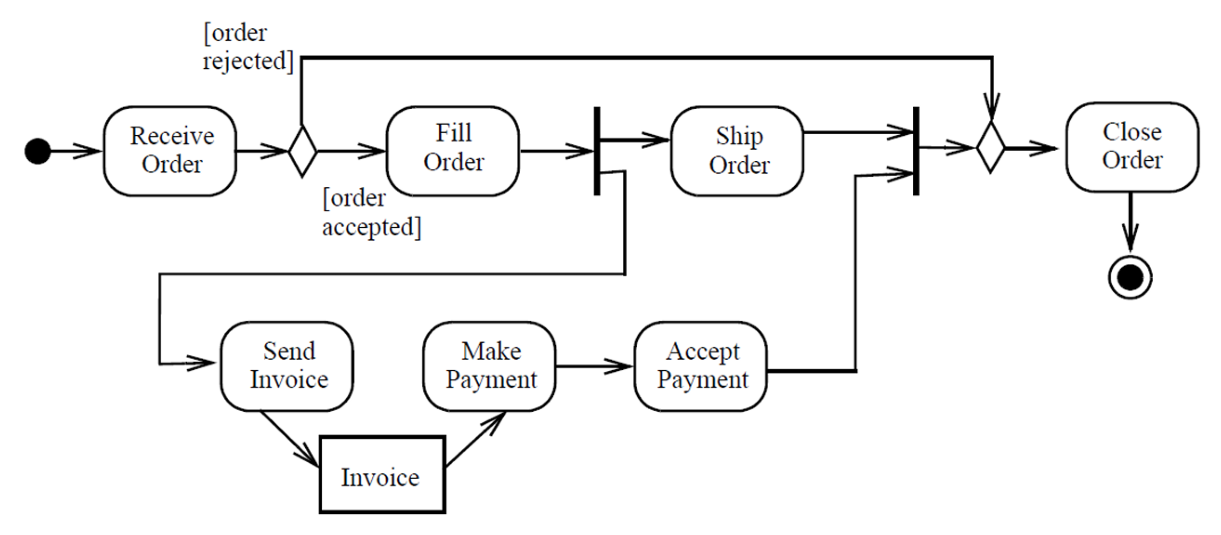
\includegraphics[scale=0.7]{orderMan_actDiagram}
	%\vspace{-0.5cm}
	\caption{The UML activity diagram for the process to handle orders, adapted from~\cite[p.~369]{omg_unified_2015}.} %
	\label{fig:orderMan_actDiagram}
\end{figure*}

Figure~\ref{fig:orderMan_actDiagram}(B) highlights for each node of the activity graph (1)~the mapping from the node to a corresponding module (\wrt the domain class referenced by the \attribn{refCls}), (2)~the out nodes (\wrt the \attribn{refCls}), and (3)~the \clazz{ModuleAct} objects each of which specifies a SAA for the behavior of the module. These \clazz{ModuleAct} objects together with SAAs are listed in Figure~\ref{fig:orderMan_unifiedModel}(C). In order to obtain an \orderman software with the GUI, as shown in Figure~\ref{fig:orderManGUI}, %
%GUIs like the one shown in Figure~\ref{fig:decisional-form-eg-gui}, 

the unified model incorporating the AGL specification (for the activity model) needs to be encoded in Java. The implemenation for \orderman is available at the git repository\footnote{\url{https://github.com/jdomainapp/orderman}}. Section~\ref{subsect:toolSupport} provides a detailed explanation of this implementation.
%
\begin{figure*}[ht]
	\centering
	\includegraphics[scale=0.355]{orderMan_unifiedModel}
	\caption{(A: Left) The activity graph whose nodes are labeled with activity and component classes; (B: Top-right) The \clazz{Node} objects; (C: Bottom-right) \clazz{ModuleAct} objects that are referenced by the \clazz{Nodes}.} %
	\label{fig:orderMan_unifiedModel}
\end{figure*}

\begin{figure*}[ht]
	\centering
	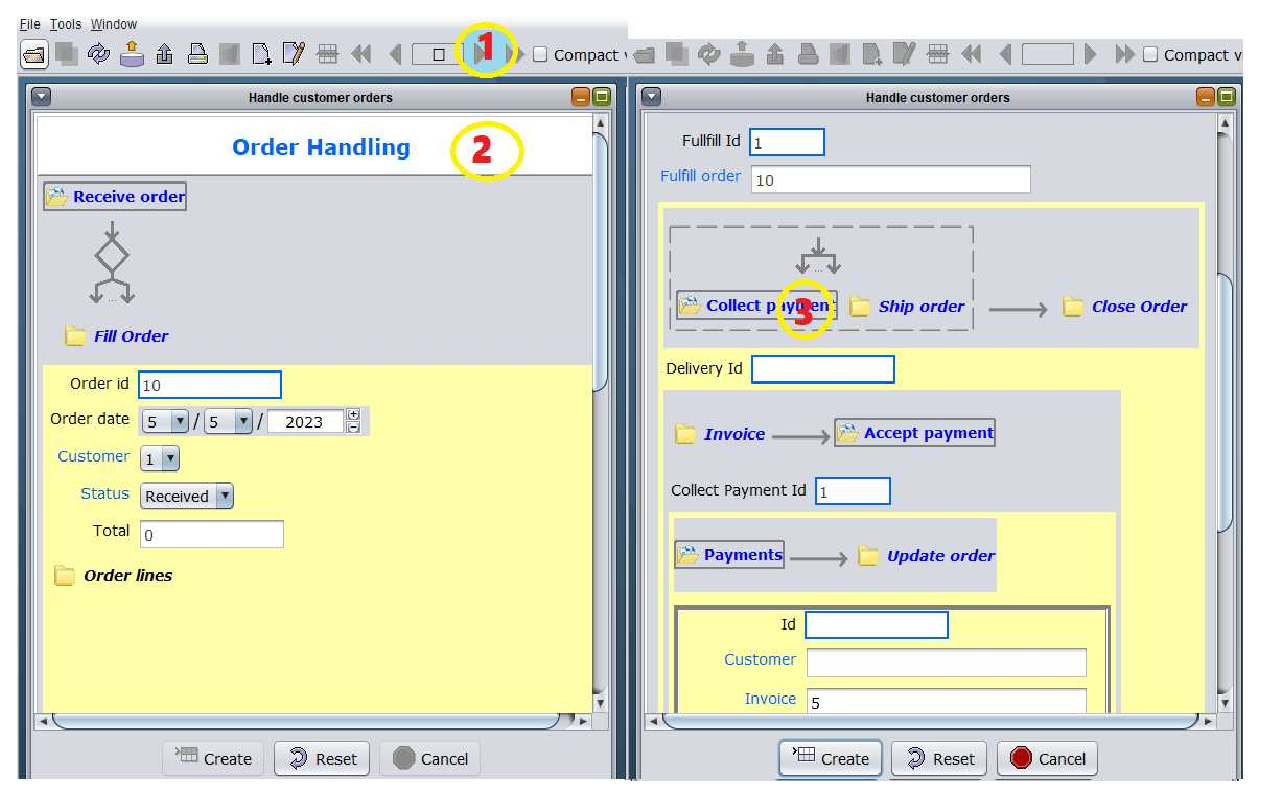
\includegraphics[scale=0.5]{orderManGUI}
	\caption{The GUI of the \orderman~software generated by the tool.} %
	\label{fig:orderManGUI}
\end{figure*}

%%%%%%%%%%%%%%%%%%%%%%%%%%%%%%%%%%%
\subsection{Tool Support}
\label{subsect:toolSupport} %
%%%%%%%%%%%%%%%%%%%%%%%%%%%%%%%%%%%%

%design choices and used technologies. For instance, this section could answer some of the following questions:
%- How annotations are inserted into Java or C code?
%- How the AGL is implemented?
%- What is the input format?

As illustrated in Figure~\ref{fig:toolSupport}, we realized our method with a support tool based on JDomainApp, a Java software framework that we reported in previous works~\cite{le_domain_2018}. The tool is available at the git repository\footnote{\url{https://github.com/jdomainapp/jda-mbsl}}. %
%
Conceptually, the tool consists of three key components: model manager, view manager, and object manager. First, the \textbf{model manager} is responsible for registering the configured unified model and making it accessible to other components 
%
in \ref{apex:agl-classOrderMan} show the activity class \clazz{HandleOrder} (Listing~\ref{lst:handleOrderClsModel}), data class \clazz{Invoice} (Listing~\ref{lst:invoiceCls}), control class \clazz{AcceptOrNot} (Listing~\ref{lst:acceptOrNotCls}) and coordinator class \clazz{FillOrder} (Listing~\ref{lst:fillOrderCls}).
%
The left window in Figure~\ref{fig:toolSupport} depicts the list of module classes (e.g., \clazz{ModuleHandleOrder}) and corresponding domain classes (i.e., \clazz{HandleOrder}). As an activity domain class the \clazz{HandleOrder} is attached with an annotation \attribn{@AGraph} for the \agl specification, as presented in the middle window in Figure~\ref{fig:toolSupport}. The annotations to realize \agl are defined by the jdomainapp framework with the java projects as shown in the left window of this figure. 

\begin{figure*}[ht]
	\centering
	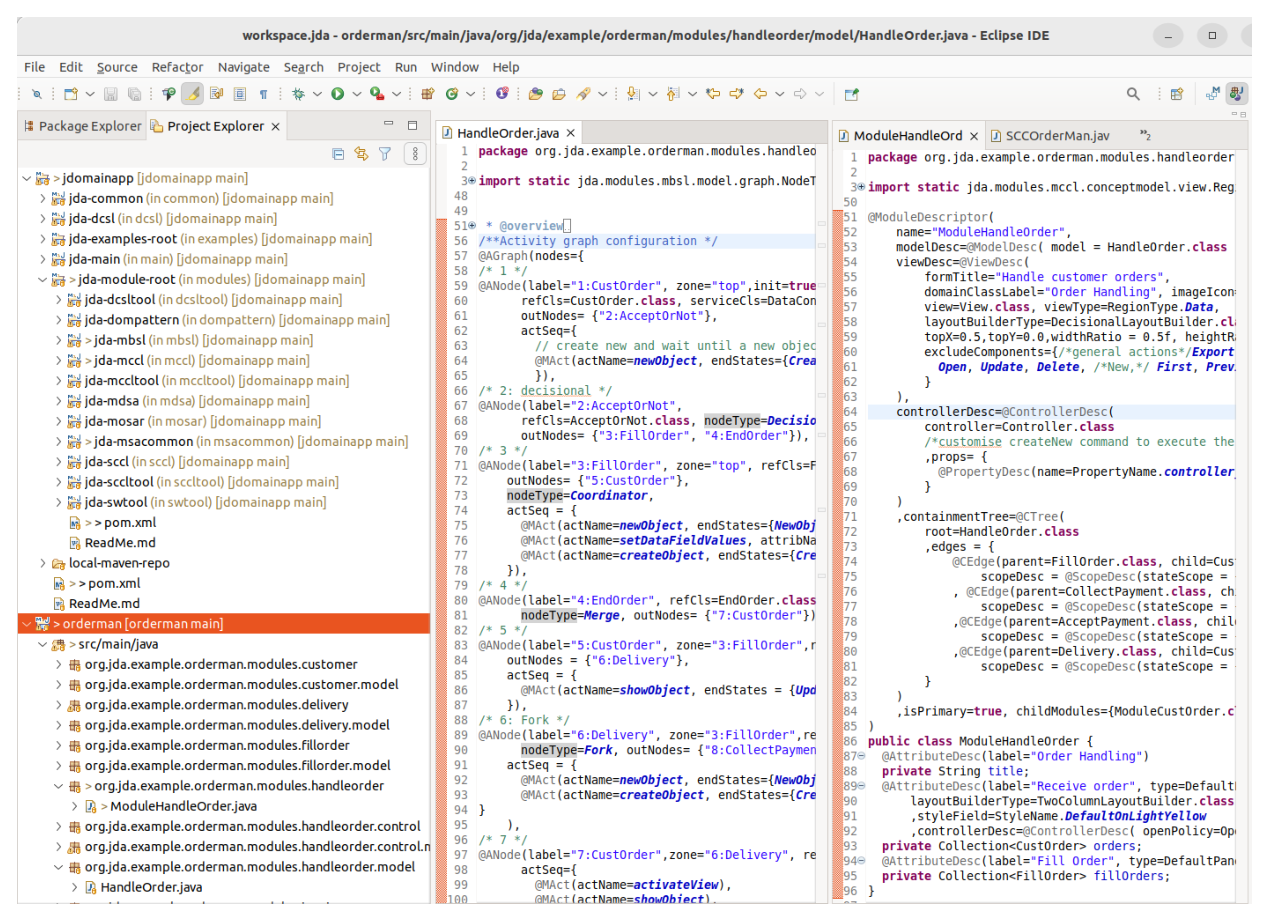
\includegraphics[scale=0.72]{toolSupport}
	\caption{Illustration for the JDomainApp-based realization and usability of \agl.} %
	\label{fig:toolSupport}
\end{figure*}

Second, the \textbf{view manager} is responsible for (1) automatically generating the entire GUI of the software from the unified model and (2) for handling the user interaction performed on this GUI. The GUI consists of a set of object UIs (one for each module's view), and a desktop for organising these UIs. The two tasks basically are based on the configuration description of modules that is specified in MCCL~\cite{le_domain_2018}. For example, the module class \clazz{ModuleHandleOrder} that owns \clazz{HandleOrder}, as presented in the right window of this figure, is specified together with a module description in MCCL.

Third, the \textbf{object manager} is responsible for managing the run-time object pool of each domain class and for providing a generic object storage component for storing (retrieving) the objects to (from) external storage. As of this writing, the tool supports both file-based and relational database storage. The relational data model is automatically generated from the unified model the first time the software is run.

\noindent\begin{minipage}{.55\textwidth}
\begin{lstcodeplainssm}{The activity class \clazz{HandleOrder} in Java}{lst:handleOrderCls}
/**Activity graph configuration in AGL */
@AGraph(nodes={...	
	/* 14 */    
	@ANode(label="14:Payment", zone="11:AcceptPayment",
		refCls=Payment.class, serviceCls=DataController.class, 
		outNodes={"15:CustOrder"},
		actSeq={
			@MAct(actName=newObject, endStates={NewObject}),
			@MAct(actName=setDataFieldValues, attribNames={"invoice"},
				endStates={Created})
		}), ...
})
/**END: activity graph configuration */
public class HandleOrder {...}
\end{lstcodeplainssm}
\end{minipage}
\begin{minipage}{.45\textwidth}
\begin{lstcodeplainssm}{Java implementation of the annotation \attribn{AGraph}}{lst:aGraphAnnotation}
package jda.modules.mbsl.model.graph.meta;

import java.lang.annotation.*;
import jda.modules.mbsl.model.graph.ActivityGraph;

@Retention(RetentionPolicy.RUNTIME)
@Target(value=java.lang.annotation.ElementType.TYPE)
@Documented
public @interface AGraph {
	ANode[] nodes();
}
\end{lstcodeplainssm}	
\end{minipage}

In the rest of this section, we would further explain how a module class \wrt an activity class can handle the execution of the activity graph \wrt its AGL specification. Let's focus on a concrete situation with the  \clazz{ModuleHandleOrder} module with its activity class, \clazz{HandleOrder}, realized as in Listing~\ref{lst:handleOrderCls}.
%
%
When the software runs, an instance of the \clazz{ModuleHandleOrder} module is invoked. Based on the configuration description of this module as shown in the right window of Figure~\ref{fig:toolSupport}, an activity model (\clazz{ActivityModel}) as a composition of the \clazz{HandleOrder} object (owned by the \clazz{ModuleHandleOrder} module) and an activity graph \wrt the AGL specification of the activity class \clazz{HandleOrder} is created. The activity diagram could be defined because the \clazz{HandleOrder} object can be considered as an \clazz{AGrap} object (based on the annotation mechanism in Java). The definition of the annotation \clazz{AGraph} is shown as in Listing~\ref{lst:aGraphAnnotation}. 
%
The \clazz{AGraph} object allows each of its \clazz{ANode}, e.g., the \clazz{ANode} \wrt node~14 as shown in Listing~\ref{lst:handleOrderCls}, as well as the domain class referenced by the \clazz{ANode} (i.e., the \clazz{Payment} class) could be handled by the \clazz{ModuleHandleOrder} module. 


























 